\documentclass[10pt,a4paper]{article}
\usepackage[margin=1.6cm]{geometry}
\usepackage{helvet}\renewcommand{\familydefault}{\sfdefault}
\usepackage{graphicx,booktabs,xcolor,fancyhdr,float,array}
\definecolor{bigorange}{RGB}{255,130,0}
\definecolor{biggrey}{RGB}{60,60,60}
\pagestyle{fancy}\fancyhf{}
\lhead{\textbf{\color{bigorange}Banco BIG} \color{biggrey}| Rates Research}
\rhead{\color{biggrey}\today}
\cfoot{\color{biggrey}\thepage}
\renewcommand{\headrulewidth}{1pt}
\setlength{\parindent}{0pt}\setlength{\parskip}{4pt}
\newcommand{\grade}[1]{{\footnotesize\color{biggrey}[#1]}}
\newcommand{\sect}[1]{\section*{\color{bigorange}#1}}
\begin{document}

% ------------------------------------------------------------------ cover
\begin{center}
{\LARGE\textbf{\color{biggrey}US Rates Research Pack}}\\[3pt]
{\color{bigorange}\rule{\textwidth}{2.5pt}}\\[3pt]
{\small Consolidated, audited session output: CFTC positioning \& curve crowding
$\cdot$ positioning$\to$yields evidence $\cdot$ US10Y forecasting (ARIMA, GBM/Heston,
walk-forward validation) $\cdot$ oil$\to$rates conditional sensitivity $\cdot$
audit of revisions. All data free/public (CFTC, FRED, NY Fed); every claim carries an
evidence grade: \grade{V} = out-of-sample validated, \grade{S} = statistically significant
(HAC), \grade{D} = descriptive only.}
\end{center}

\sect{1. Executive summary --- verified headlines}
\begin{tabular}{p{8.6cm}p{4.4cm}l}
\toprule
Claim & Value & Grade\\
\midrule
Positioning: crowded net-LONG duration extreme & composite $z=+2.49$, 89.7th pctile (2026-07-14) & \grade{D}\\
\quad driver: asset managers long the long end; dealers mirror-short & AM $z$ $+1.21$; lev funds $-0.25$ & \grade{D}\\
Crowded-long extremes preceded higher yields\ldots & P(up) 0.53/0.63/0.66/0.74 at 4/8/13/26w & \grade{D}\\
\quad \ldots but NOT statistically robust & all 95\% CIs include 0.5; Granger $p{\ge}0.80$ & \grade{S-tested, fails}\\
US10Y point forecasting: nothing beats a random walk & ARIMA/RW RMSE 0.9985, DM $p{=}0.62$ & \grade{V}\\
30-day fan (validated widths, zero drift) & median 4.62\%, 90\% [4.24, 5.05], P(up) 49\% & \grade{V (coverage)}\\
\quad trend drift is WORSE than zero drift OOS & RMSE 0.316 vs 0.287, DM $p{=}0.07$ & \grade{V}\\
\quad all fan conditioning rejected OOS at 30d & CRPS 16.05bp base vs 16.05--16.20 variants & \grade{V}\\
Desk: barrier / tail numbers (10k paths) & P(touch 5.00\%)=11\%, P(touch 4.25\%)=9\%; 10M 10y VaR95 $-$330k & \grade{V (widths)}\\
Oil moves rates only via breakevens, and barely & $\beta_{10y}=+0.26$bp/1\% ($t{=}6.6$, $R^2{=}1.4\%$); real leg $t{=}0.4$ & \grade{S}\\
\quad big-oil days: real \& breakeven legs offset & opposite signs 60\% of days, $|$real$|$ larger & \grade{D}\\
\quad sensitivity saturates with oil vol & interaction $t{=}-5.0$; $|$oil$|{>}5\%$ days: mean $\Delta y=-0.7$bp & \grade{S}\\
\quad demand-day beta significant, supply-day not & $+0.215$ ($t{=}2.6$) vs $+0.132$ ($t{=}1.6$), 2016+ & \grade{S / fails}\\
Curve books are FLAT in raw DV01 (both categories) & lev $-0.1$, AM $-5.0$ \$mm/bp front$-$long & \grade{D}\\
\quad the $+1.46$ ``steepener'' $z$ = unwind momentum, not a book & raw flat; $z$ vs 3y history & \grade{D, corrected}\\
\bottomrule
\end{tabular}

\vspace{4pt}
\textbf{One-line outlook.} No honest directional edge on the 10Y over 30 days
(P(up)${\approx}$49--50\% from every validated model); the crowding backdrop leans
selloff \grade{D}; the validated uncertainty band is 4.24--5.05\%; oil is a second-order
input on a mixed/supply tape; curve positioning is momentum-steepening but books are flat.

\begin{figure}[H]\centering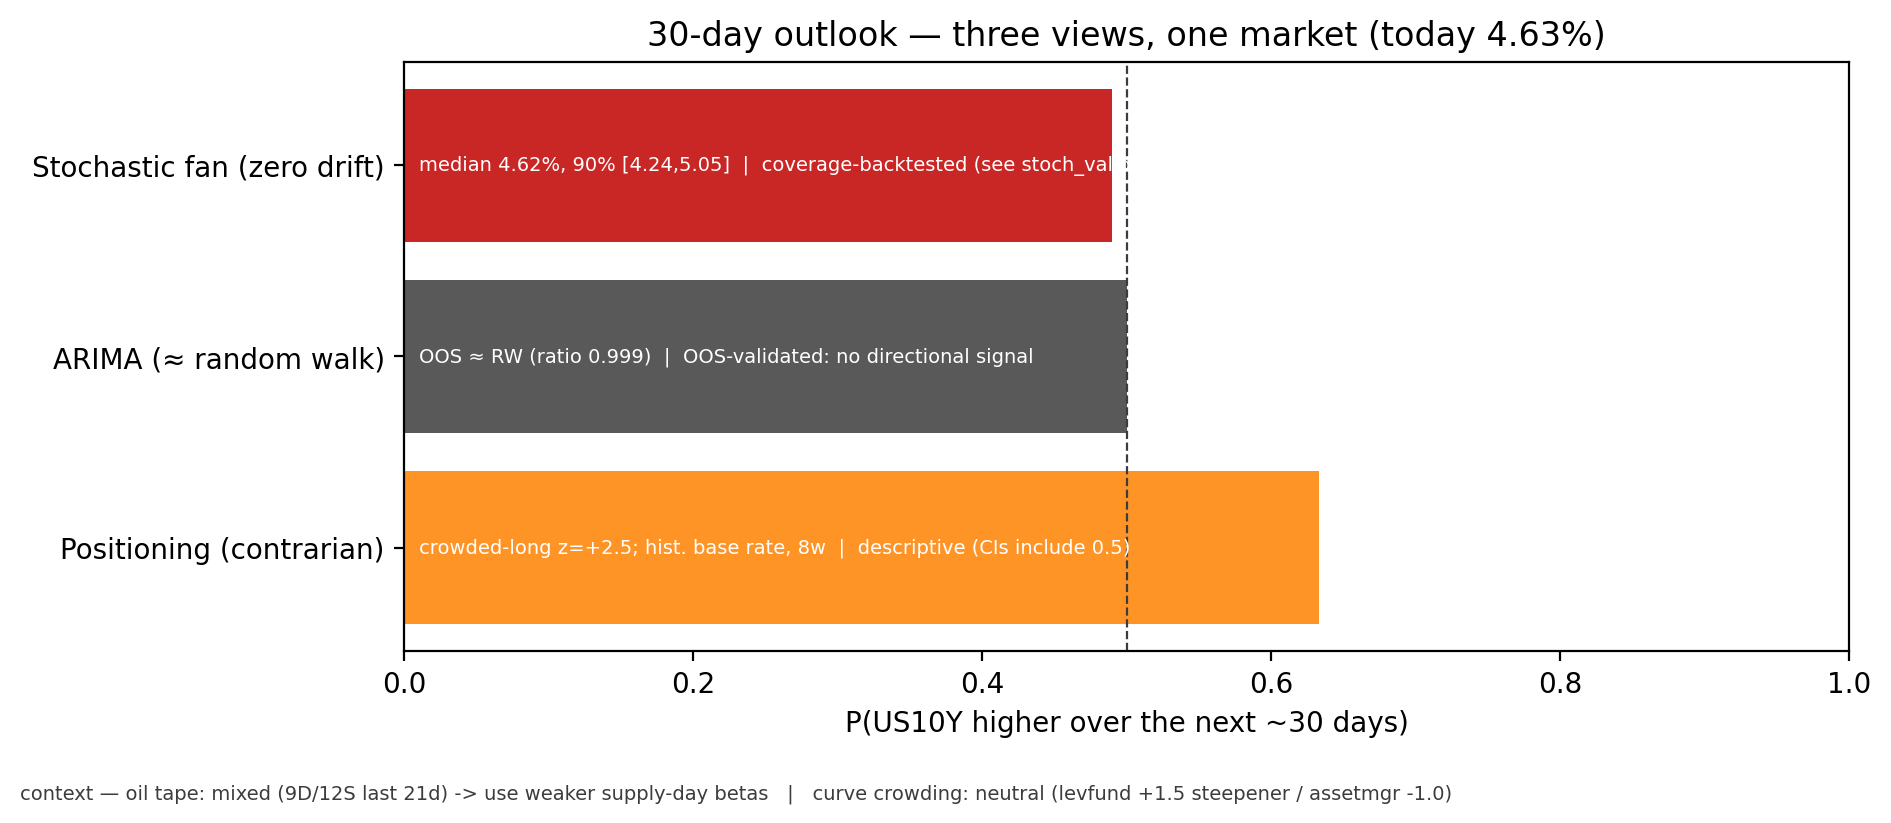
\includegraphics[width=0.9\textwidth]{../results_rates_study/fig_outlook.png}\end{figure}

\sect{2. Positioning: crowding score and curve read}
\textbf{Method.} CFTC TFF net positions (TU/FV/TY/TN/US/UB) $\to$ DV01 $\to$ per-category
z-scores $\to$ PCA composite (crowding $z$; $+$ = crowded net long duration). Causal
publication-lagged timeline throughout; predictive overlay embargo-purged (leakage-free
walk-forward AUC 0.554 --- weak, treated as context only).

\textbf{Current read (2026-07-14).} Composite $z=+2.49$ (89.7th pctile), a multi-year
crowded-long extreme; asset managers carry it (long TY/TN/UB), dealers mirror-short,
lev funds $\approx$ neutral outright. Stance: contrarian short-duration \grade{D}.

\begin{figure}[H]\centering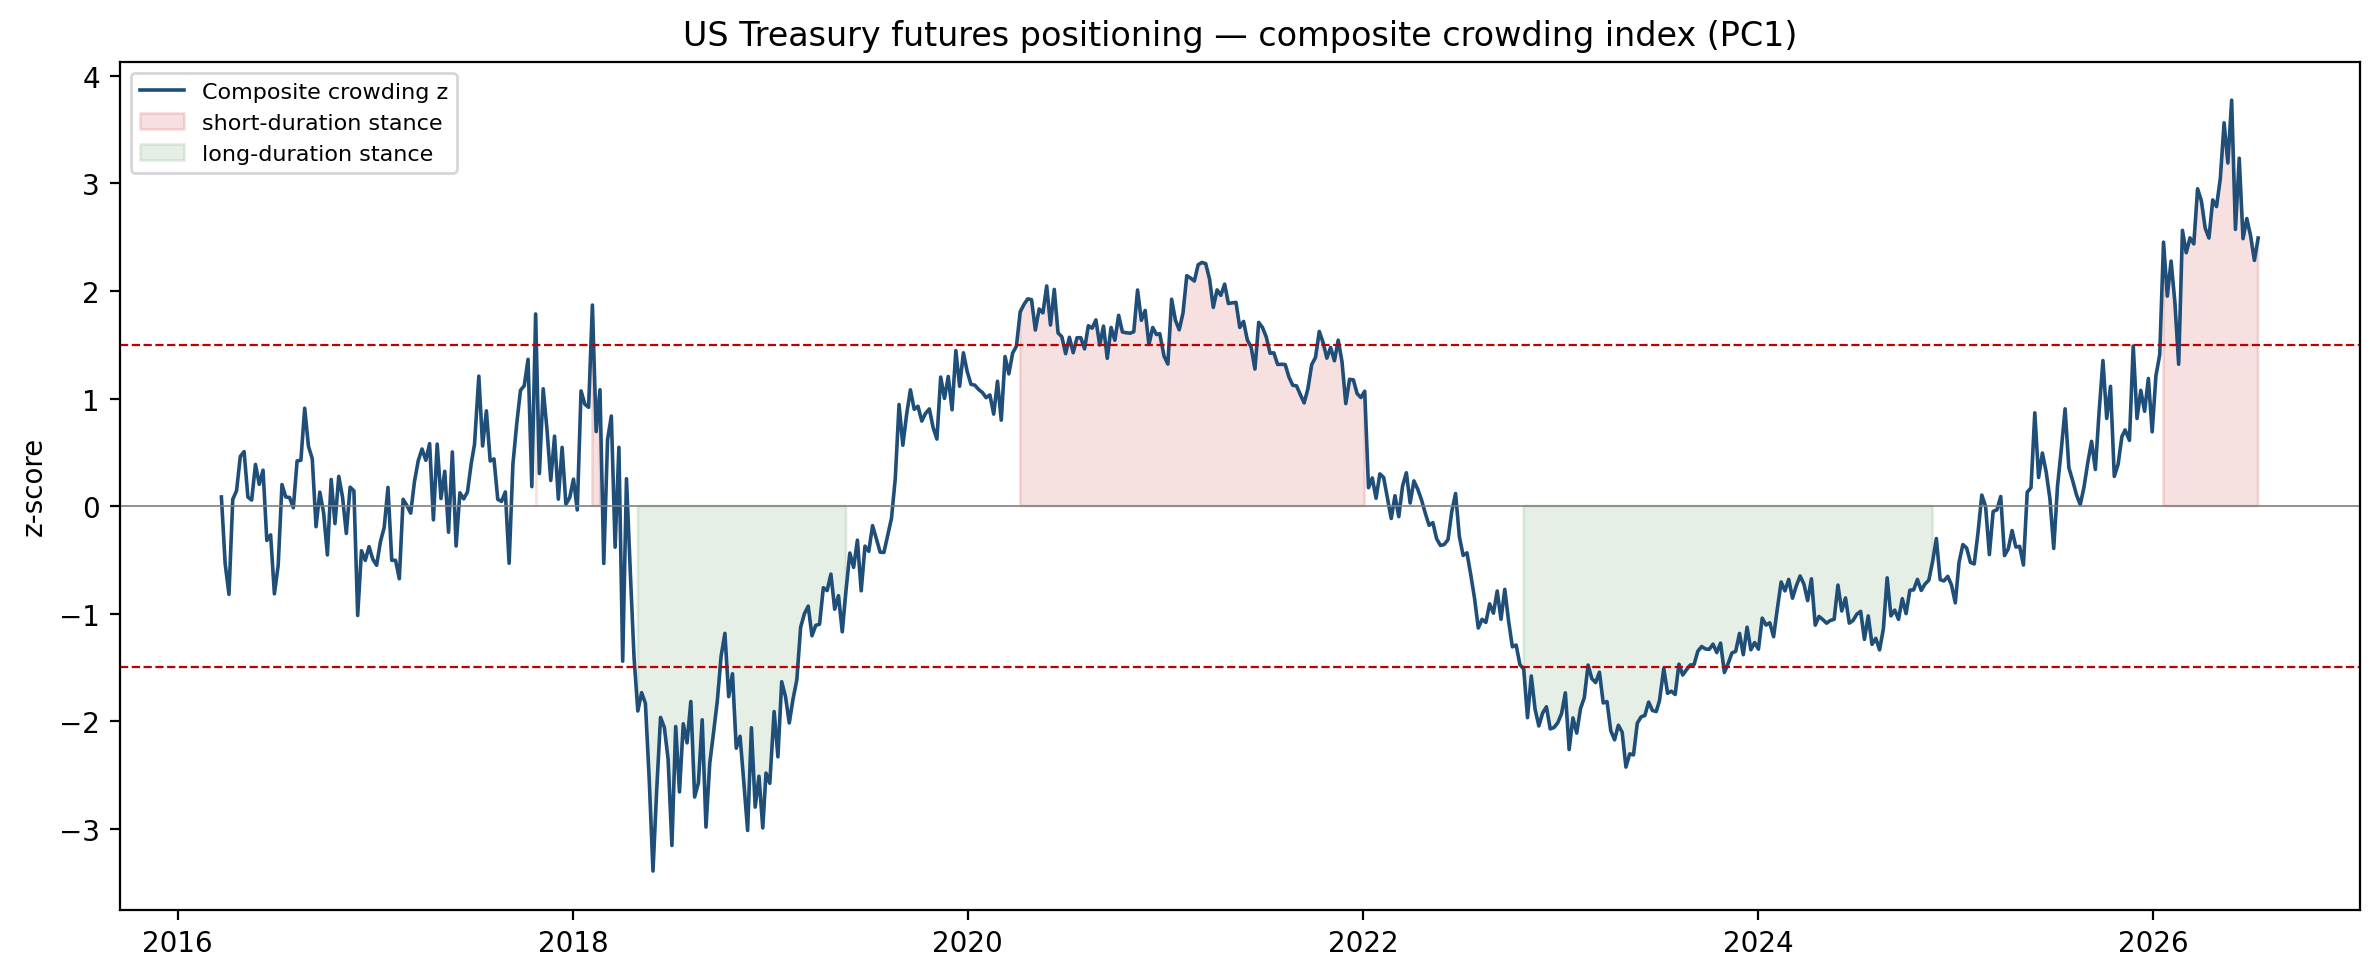
\includegraphics[width=0.95\textwidth]{../positioning/results/fig_positioning_composite.png}\end{figure}
\begin{figure}[H]\centering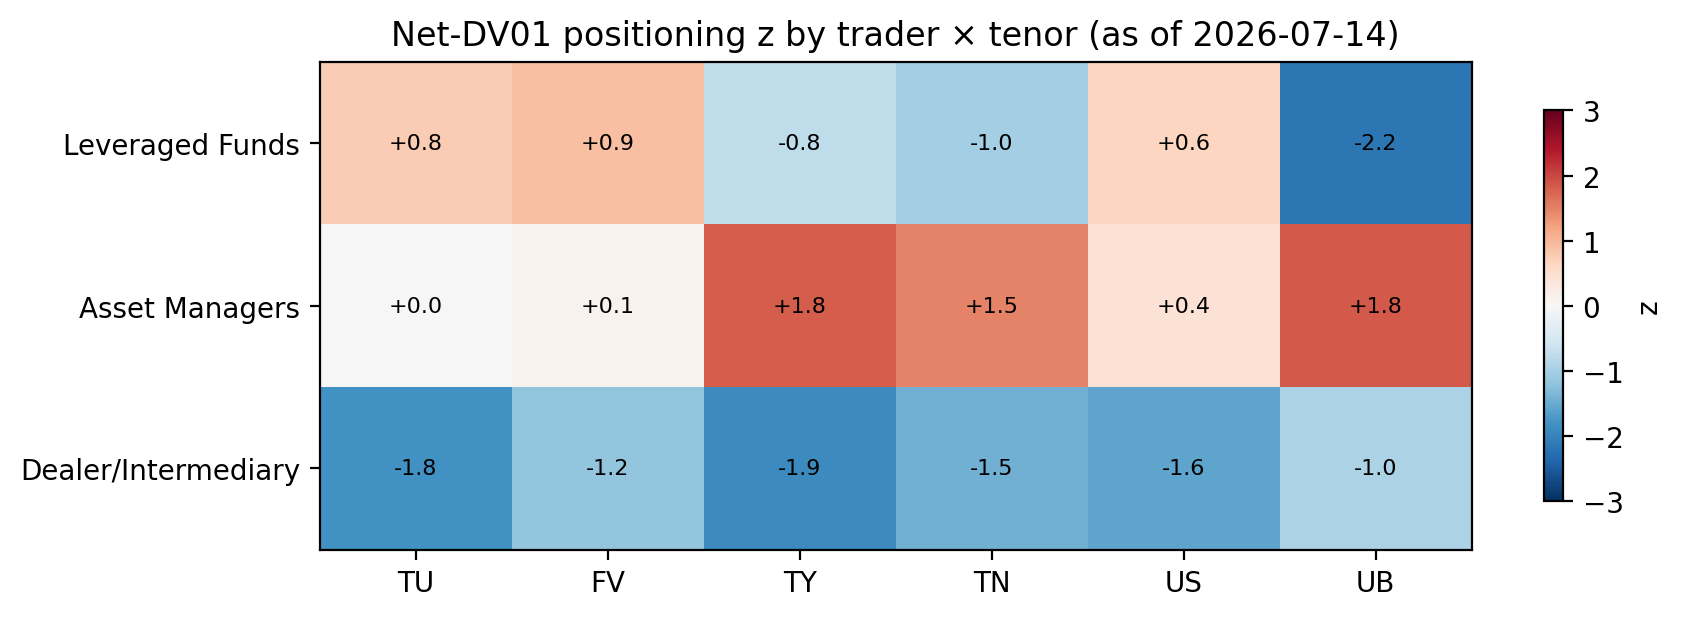
\includegraphics[width=0.85\textwidth]{../positioning/results/fig_positioning_heatmap.png}\end{figure}

\textbf{Curve positioning --- the corrected two-dimension read.} The per-category curve
$z$ (front TU+FV minus long US+UB net DV01, vs 3y history) shows lev funds at $+1.46$;
but the RAW books are flat: lev funds front $-150.9$ vs long $-150.8$ \$mm/bp
(difference $-0.1$); asset managers $+188.4$ vs $+193.5$ ($-5.0$). The $z$ therefore
measures the sharpest steepener-DIRECTION unwind in 3 years (from a large 2022--24
flattener book back to flat), not a crowded steepener stock. Historically, extremes of
this $z$ preceded curve FLATTENING (P(flatten$|$steepener-$z{>}1.5$) = 0.74/0.80/0.78 at
4/8/13w, mean $-7/-13/-20$bp; flattener-$z$ extremes showed continuation, 0.57--0.65)
--- a positioning-momentum-exhaustion pattern \grade{D: full-sample, clustered episodes}.

\begin{figure}[H]\centering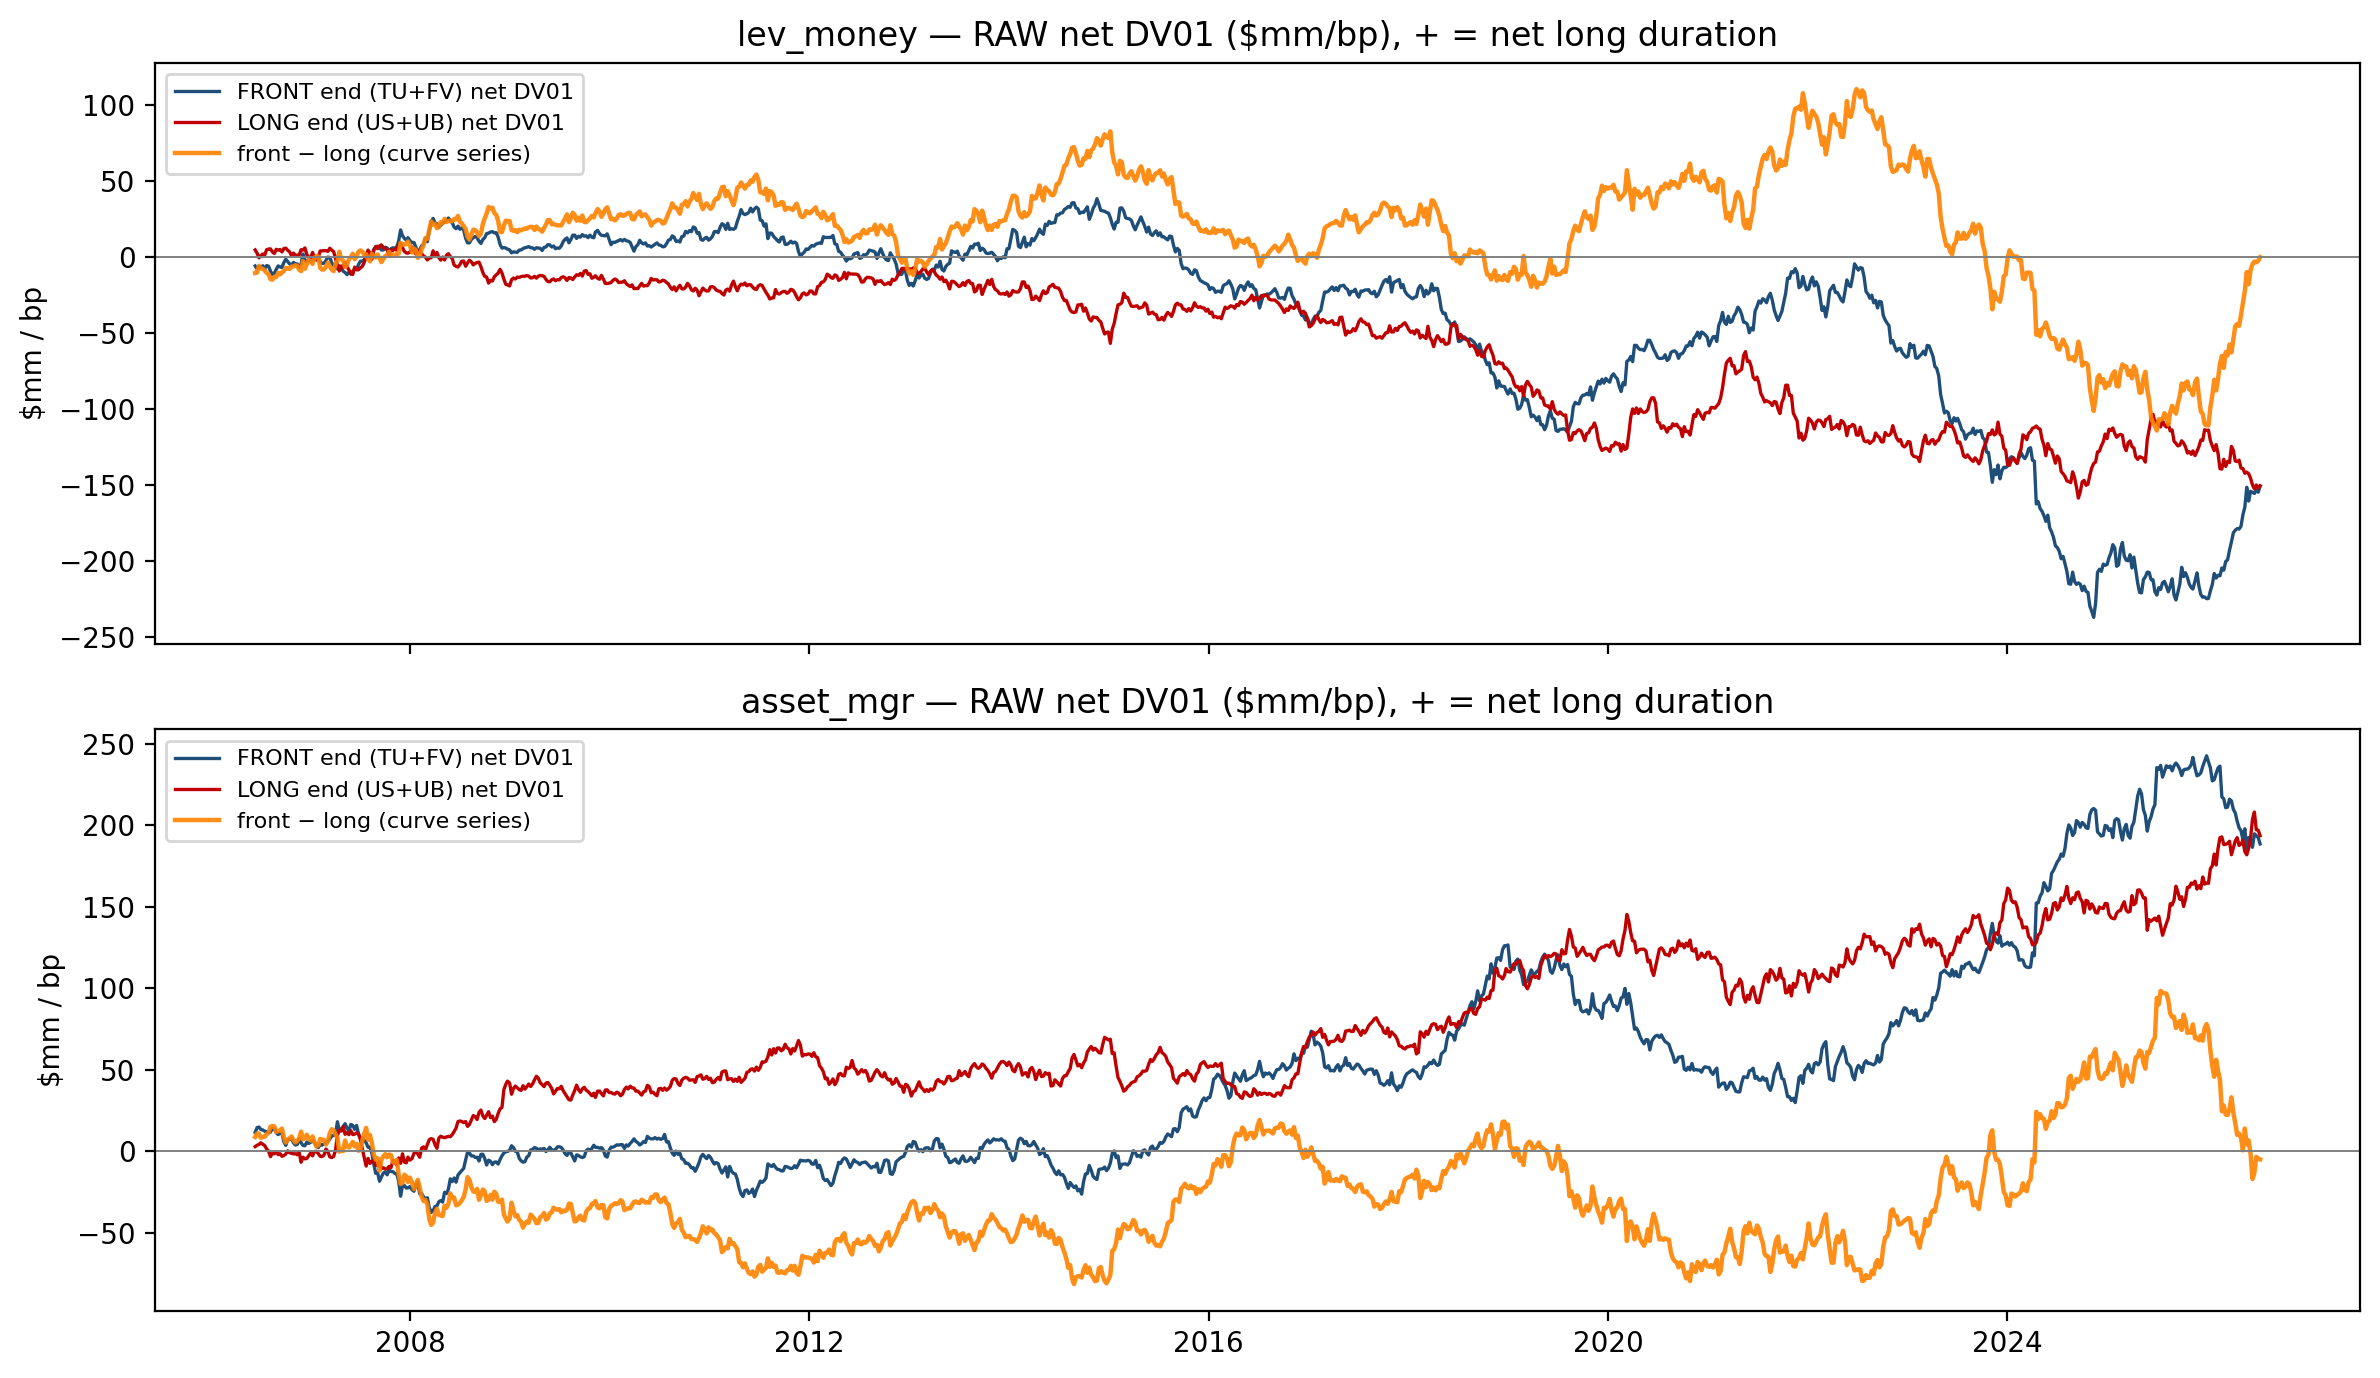
\includegraphics[width=0.95\textwidth]{../positioning/results/fig_curve_raw_dv01.png}\end{figure}

\sect{3. Does crowded positioning predict yields? (the honest evidence)}
Point estimates lean contrarian and strengthen with horizon (table), but the effect is
NOT statistically robust: block-bootstrap CIs include 0.5 at every horizon, Granger
causality is absent ($p=0.80$--$0.95$), Newey--West forward regressions are weak
($t=0.3$--$1.1$, $R^2 \le 3.5\%$), and the crowded weeks form few independent episodes
(the current one is 21 consecutive weeks). Sub-period analysis concentrates the effect
in 2020--22 and 2023--26.

\begin{center}\begin{tabular}{lccccc}
\toprule
Horizon & n & P(yield up) & 95\% CI & mean $\Delta y$ & unconditional\\
\midrule
4w  & 83 & 0.53 & [0.37, 0.67] & $+3.7$bp & 0.51\\
8w  & 79 & 0.63 & [0.41, 0.86] & $+7.9$bp & 0.56\\
13w & 74 & 0.66 & [0.38, 0.91] & $+14.1$bp & 0.57\\
26w & 62 & 0.74 & [0.48, 1.00] & $+32.9$bp & 0.57\\
\bottomrule
\end{tabular}\end{center}

\begin{figure}[H]\centering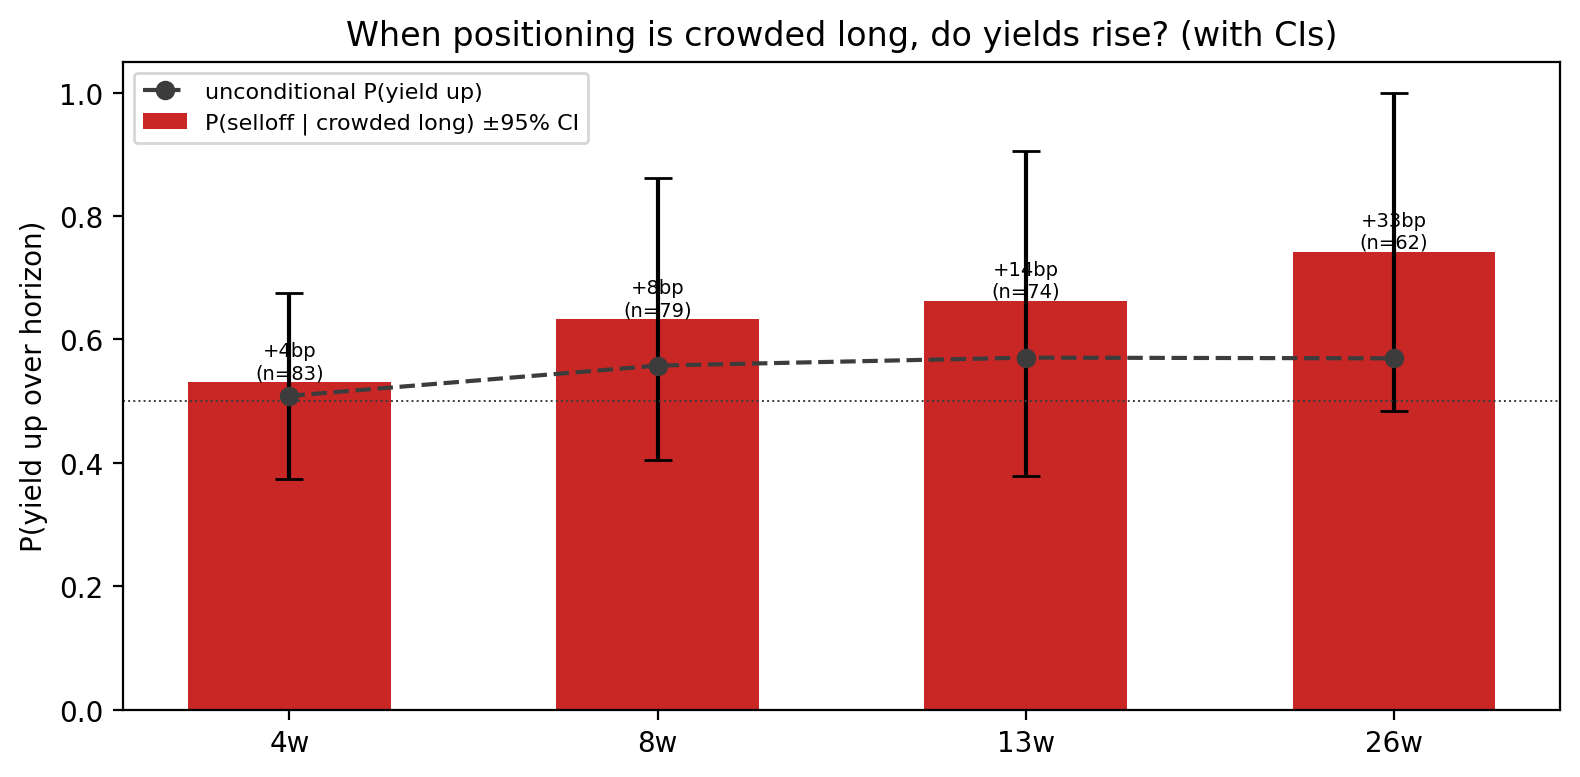
\includegraphics[width=0.8\textwidth]{../results_rates_study/fig_conditional.png}\end{figure}

\sect{4. US10Y forecasting: ARIMA, stochastic fan, and the validation program}
\textbf{ARIMA \grade{V}.} DGS10 is I(1); recursive walk-forward ARIMA(0,1,2)
one-step OOS RMSE ratio vs random walk = 0.9985 (DM $p=0.62$): indistinguishable from RW.
Adding the positioning composite as ARIMAX exogenous input does not help (ratio 0.9993,
DM $p=0.80$).

\textbf{Stochastic fan \grade{V for widths}.} The yield is modelled as an asset price
(GBM / Heston SV, 10{,}000 antithetic paths, 30bd). Heston parameters are mapped from a
GARCH(1,1) MLE ($v_0$ = the filter's current conditional variance: 15.1\%/y ann.\ vol;
long-run 16.9\%/y; $\kappa\approx0.5$/y; $\rho=-0.08$). Walk-forward validation at 125
non-overlapping origins (2011--2026):
\begin{itemize}\itemsep1pt
\item \textbf{Coverage is honest}: the 90\% band covered 89.6\% of realized 30bd outcomes
(Kupiec $p=0.88$); PIT uniform (KS $p=0.65$).
\item \textbf{Drift: zero (RW) wins}; the since-Dec-2025 trend drift is the WORST
candidate (RMSE 0.316 vs 0.287; DM $p=0.072$; its P(up) Brier 0.295 is worse than
know-nothing 0.25). The earlier trend-drift headline ``P(up)=70\%'' is retracted;
the validated number is 49\%.
\item \textbf{All conditioning rejected at 30d} (CRPS scoreboard): positioning tilt
(16.05bp, no gain; active 18/125 origins), stress widening (16.12, worse ---
GARCH $v_0$ already carries the vol state), calendar/event vol (16.06, diluted at
${\sim}3$ event days of 30; expected to matter at 1w), Vasicek (equal CRPS but
under-covers 0.87), CIR (16.20). The base fan is a proven local optimum at this horizon.
\end{itemize}

\begin{figure}[H]\centering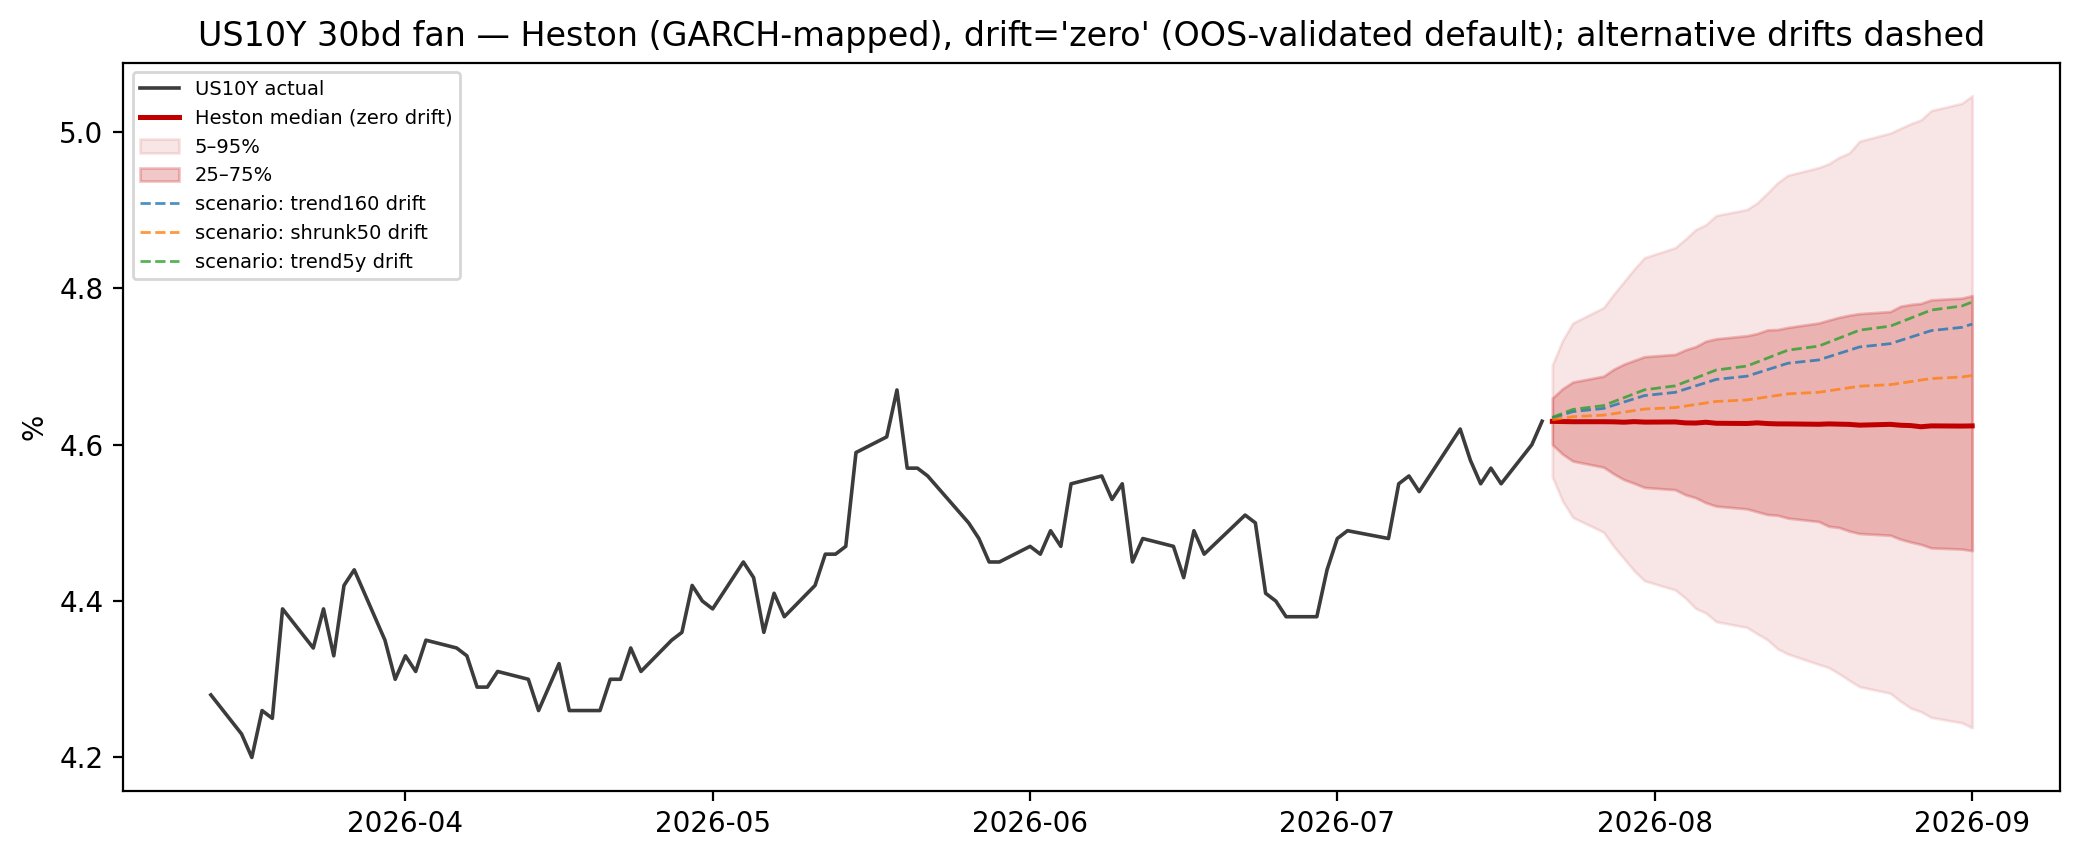
\includegraphics[width=0.95\textwidth]{../results_rates_study/fig_heston_fan.png}\end{figure}
\begin{figure}[H]\centering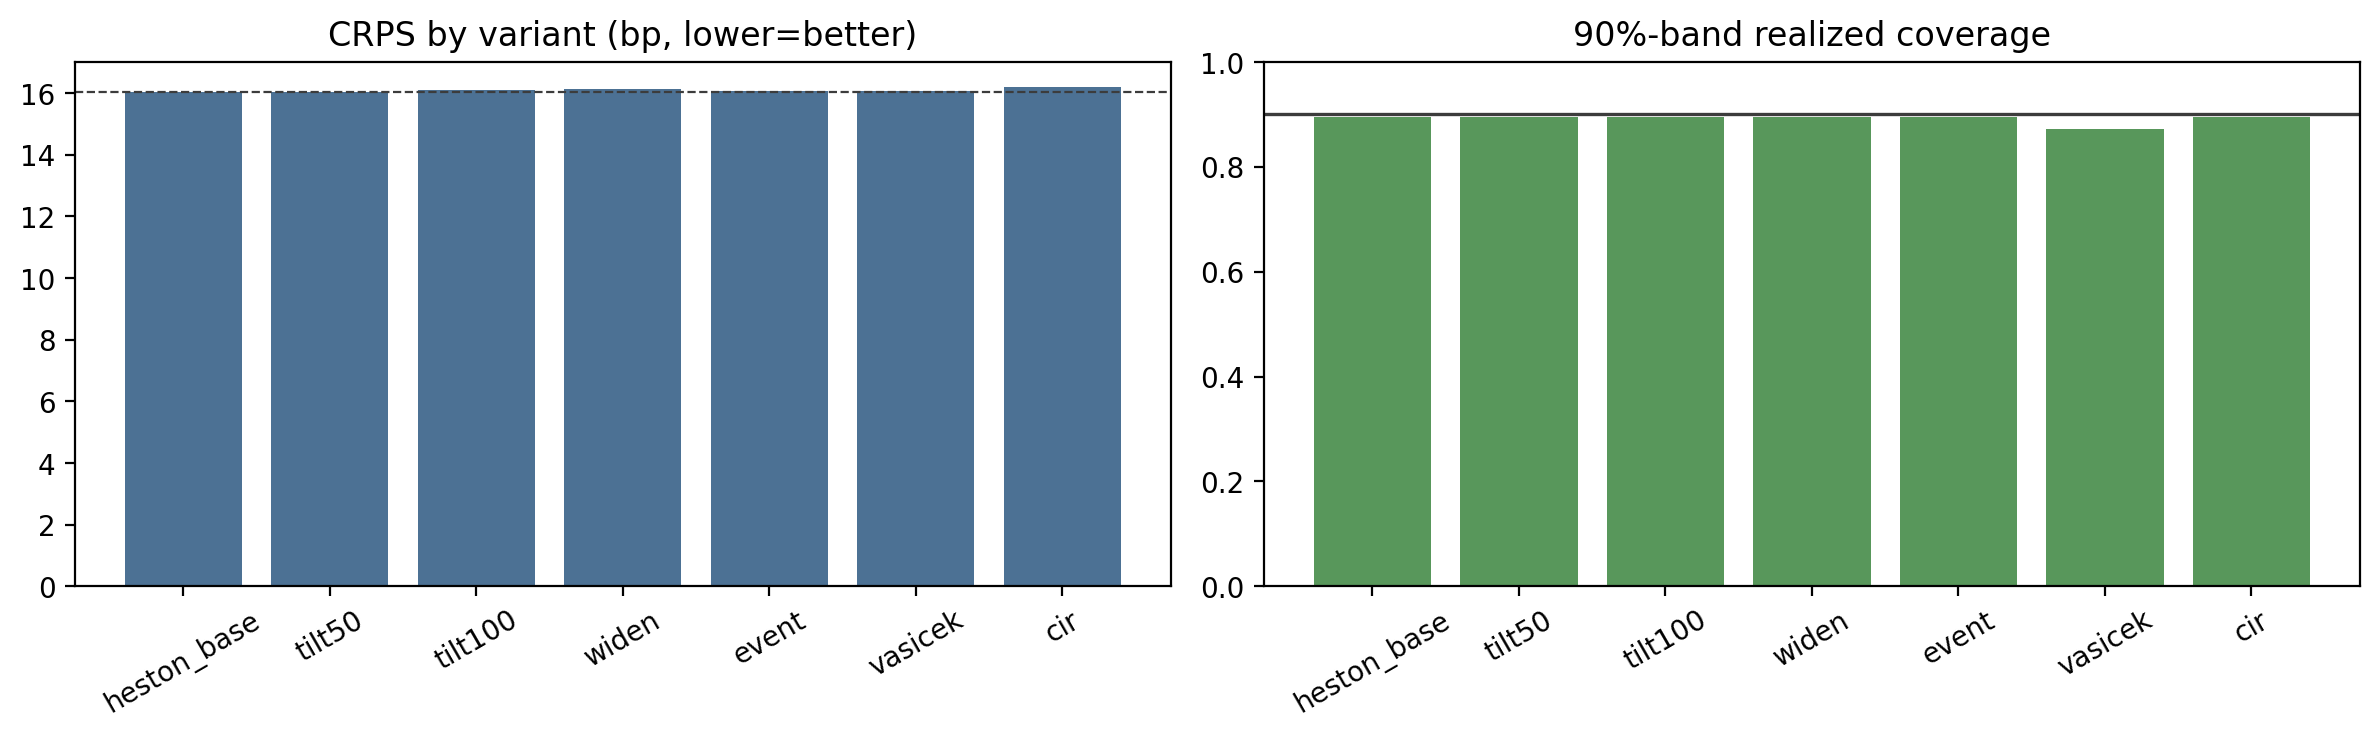
\includegraphics[width=0.95\textwidth]{../results_rates_study/fig_variant_scoreboard.png}\end{figure}

\textbf{Desk numbers (from the validated fan).} Day-30 median 4.62\%
($\pm0.2$bp MC s.e.), 90\% band [4.24, 5.05]\%; P(touch 5.00\%)=10.8\%,
P(touch 4.25\%)=8.6\%; long 10y 10M notional 30d VaR95 $\approx-330$k (DV01
${\sim}$793/bp per 1M). Mean-reversion benchmark: Vasicek half-life 182d toward
$\theta=4.35\%$ (under-covers OOS; kept as comparator, not default).

\sect{5. Oil and rates: a conditional, channel-specific relationship}
\textbf{The puzzle quantified \grade{S}.} Daily $\beta(\Delta y_{10}\!\sim\!$oil$)=+0.26$bp
per 1\% ($t=6.6$) but $R^2=1.4\%$: a 5\% oil move maps to ${\sim}1.3$bp. Monthly
$+0.36$ ($t=2.6$); Brent similar.

\textbf{Mechanism: offsetting channels \grade{S}.} The entire nominal effect runs through
breakevens ($\beta_{BEI}=+0.27$, $t=4.2$, $R^2=5.3\%$); the real leg is nil on average
($t=0.4$). Granger: oil$\to$BEI $p=0.003$; oil$\to$real $p=0.44$; strong reverse
feedback rates$\to$oil ($p\approx0$). On $|$oil$|>3\%$ days ($n=737$) the two legs move
in OPPOSITE directions 60\% of the time (corr $-0.32$) with the real leg larger
(4.7 vs 3.5bp): the growth channel cancels the inflation channel exactly when oil moves
most.

\begin{figure}[H]\centering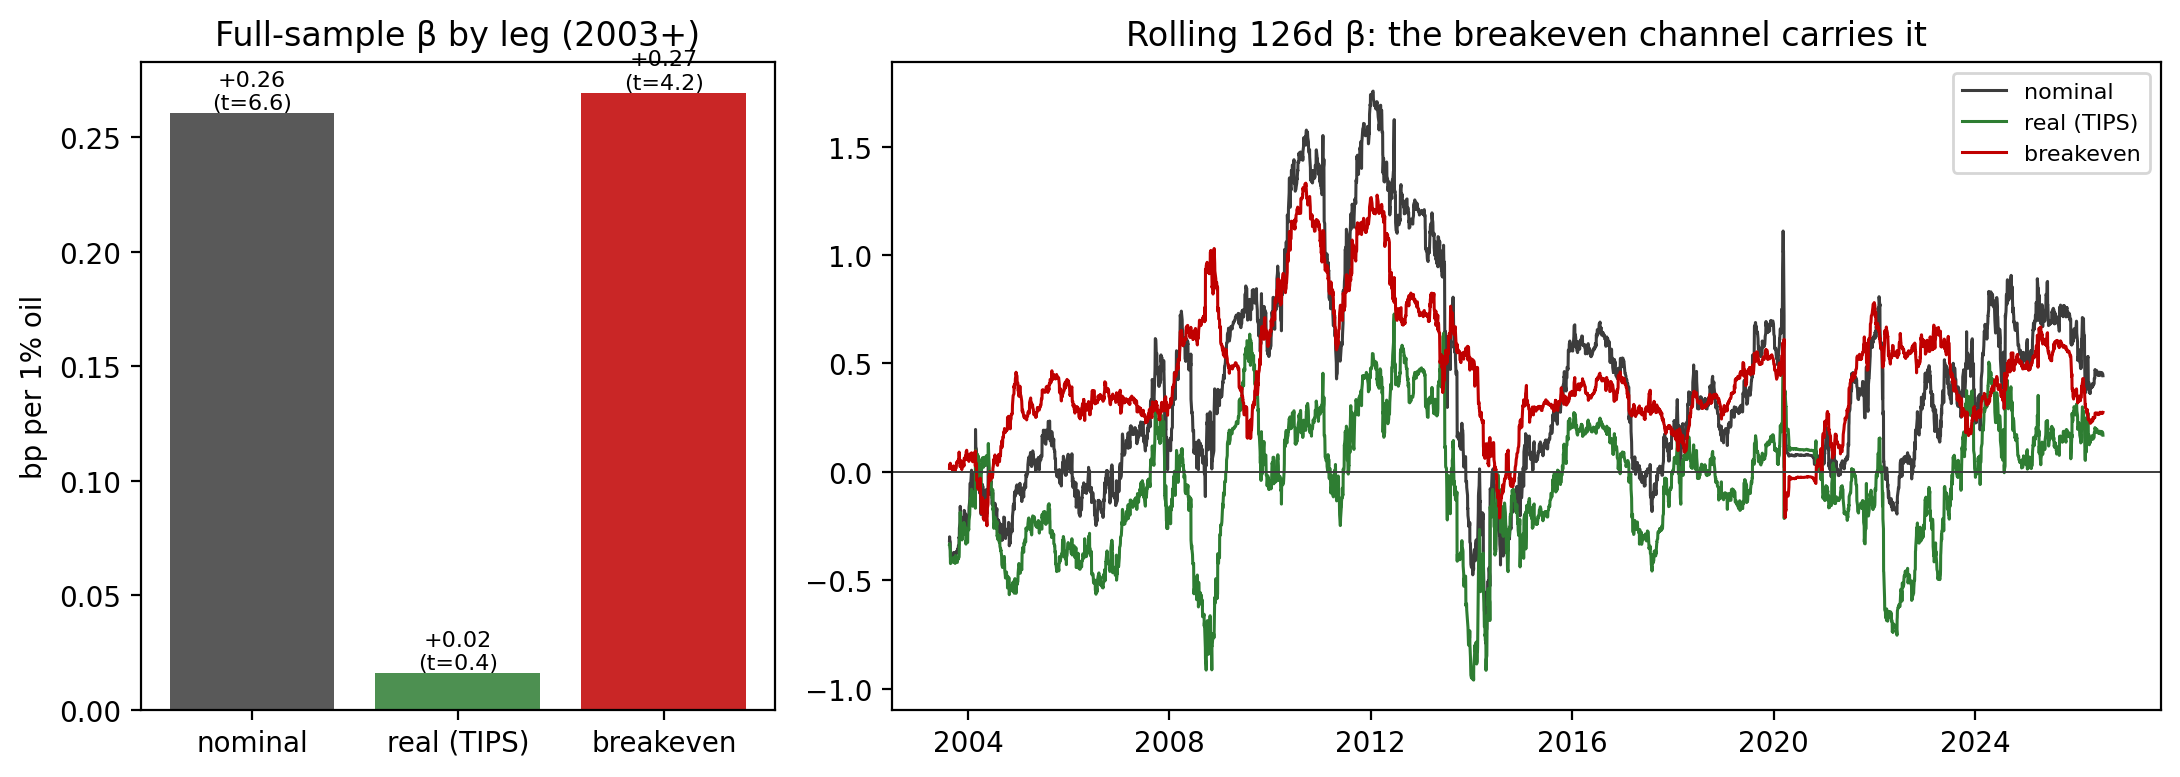
\includegraphics[width=0.95\textwidth]{../results_oil_rates/fig_decomposition.png}\end{figure}

\textbf{Regimes and saturation \grade{S}.} A 2-state Markov switch puts the LOW-beta
state ($\beta=0.21$, 37\% of days, $\sigma=8$bp/d) in high-stress conditions (VIX 23 vs
17; elevated oil and rate vol; fires in 2008--09, 2011--12, 2020, 2022--23); the calm
state carries $\beta=0.33$. The only significant interaction is oil volatility
($t=-5.0$): per-unit sensitivity roughly halves as oil vol doubles, so bp-response is
nearly regime-invariant (${\sim}0.55$--$0.68$bp/day) --- the response SATURATES.

\textbf{Shock type (2016--2026, FRED SP500 classifier) \grade{S/fails}.} Demand-day
$\beta=+0.215$ ($t=2.64$, significant, via breakevens); supply-day $\beta=+0.132$
($t=1.61$, indistinguishable from zero); ordering as hypothesized but the magnitude gap
is modest --- the sharp distinction is significance. Current 21d tape: 9 demand / 12
supply = mixed $\Rightarrow$ apply the weak supply-day betas.

\textbf{Datapoints that skew the fit \grade{D}.} Cook's-distance leaders are supply/panic
days --- 2020-04-21 (oil $-72\%$, rates $-5$bp), 2020-03-18 ($-27.5\%$, $+16$bp
wrong-signed), 1991-01-17 (Gulf War), Nov-2008 --- and they DRAG the unconditional beta
DOWN: OLS $+0.261 \to +0.298$ excluding the top-1\% Cook's D (Huber $+0.267$).
Conditional on $|$oil$|>5\%$ ($n=349$): mean $\Delta y_{10} = -0.7$bp $\approx$ 0.
(The 2020-04-20 negative-WTI print is excluded from returns by construction.)

\begin{figure}[H]\centering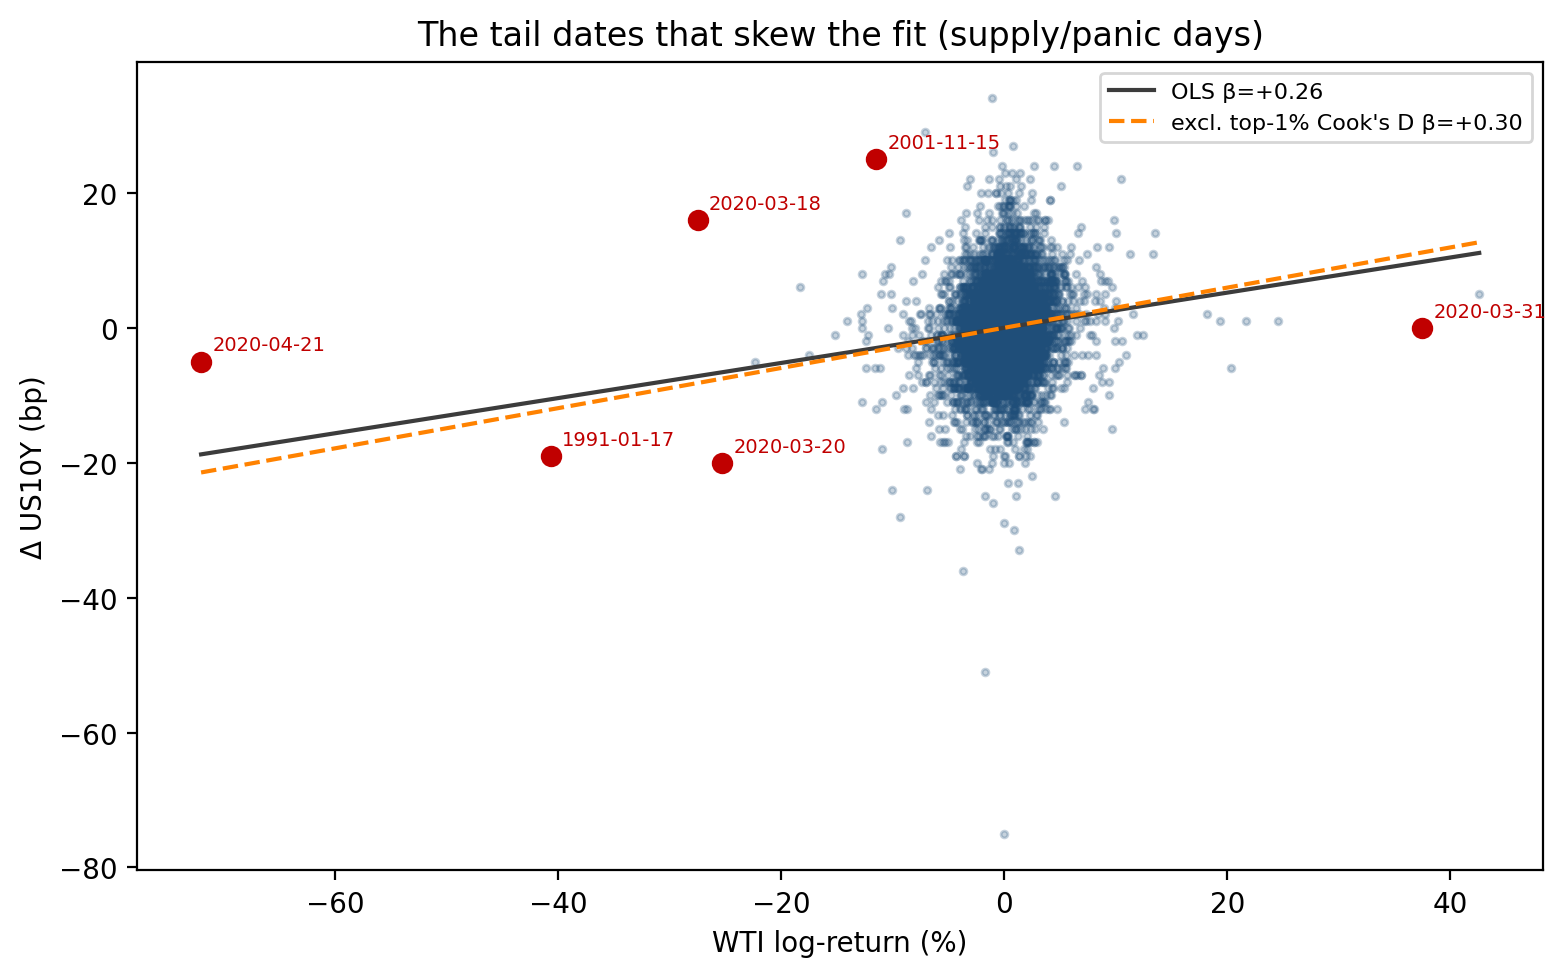
\includegraphics[width=0.62\textwidth]{../results_oil_rates/fig_influence.png}\end{figure}
\begin{figure}[H]\centering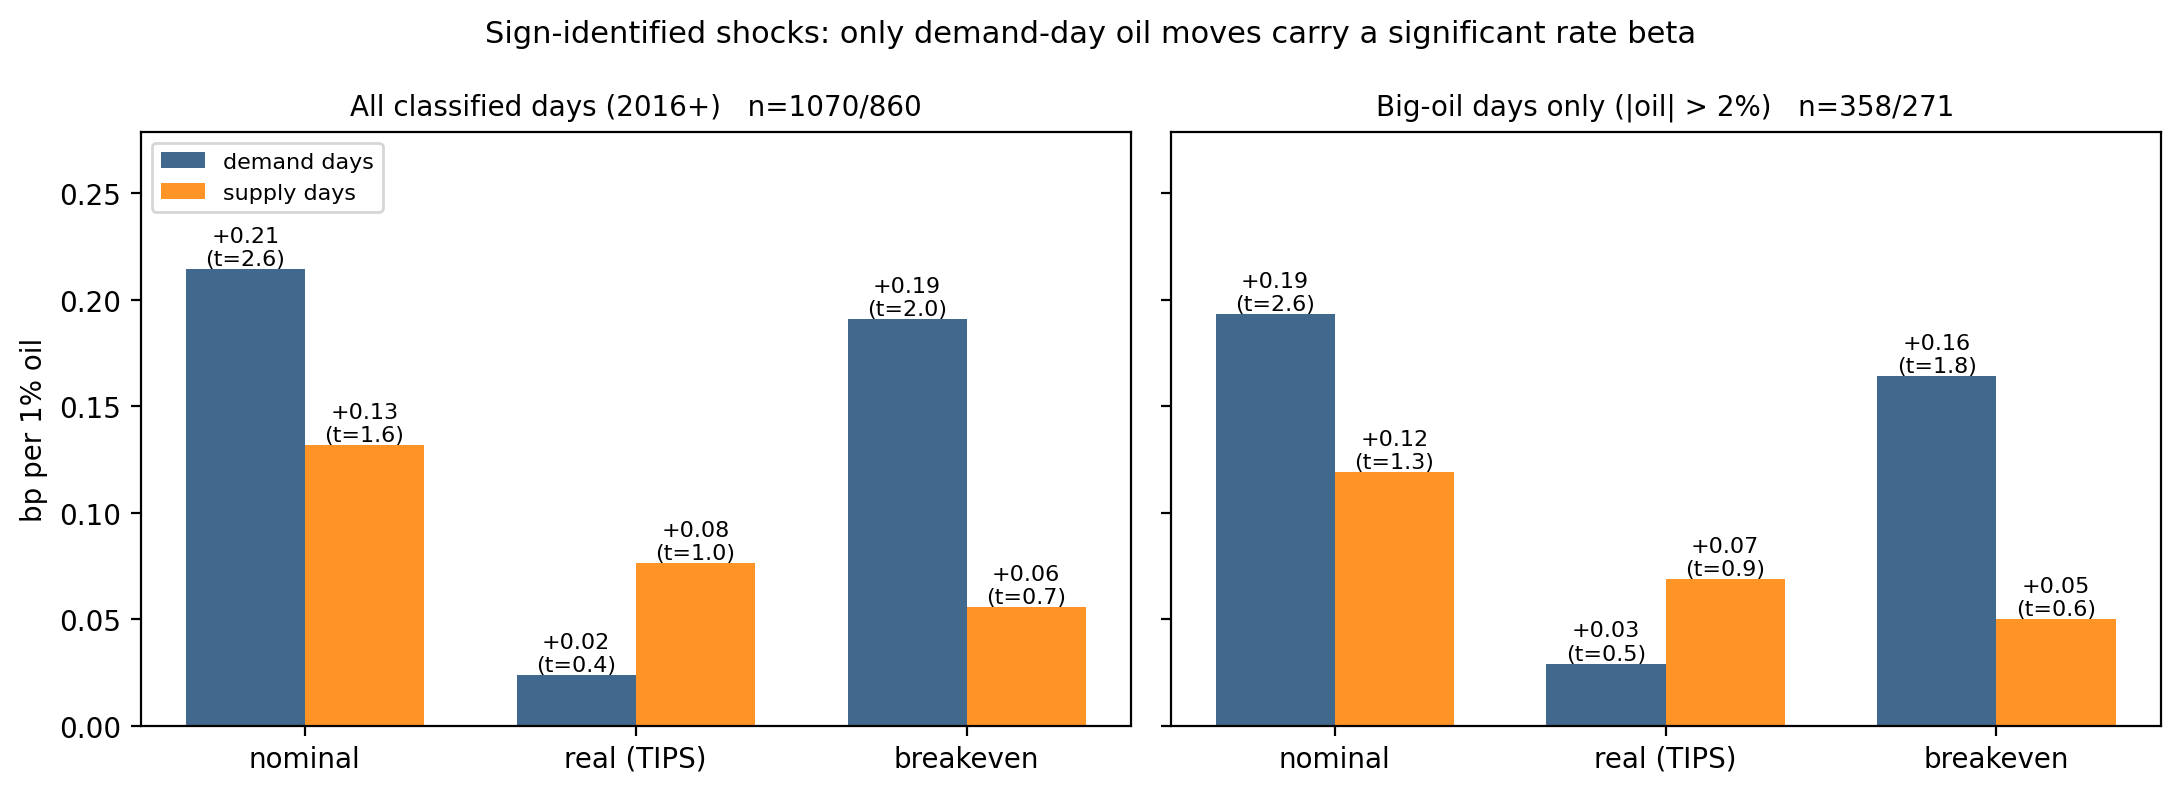
\includegraphics[width=0.8\textwidth]{../results_oil_rates/fig_shock_type.png}\end{figure}

\sect{6. Audit: inconsistencies found and resolutions}
\begin{enumerate}\itemsep2pt
\item \textbf{P(up) 70\% $\to$ 49\% (retraction).} The first fan used the since-Dec-2025
trend drift; walk-forward validation showed that drift is WORSE than zero OOS
(DM $p=0.07$). The validated headline is P(up)=49\%.
\item \textbf{``Crowded steepener'' $\to$ momentum, flat book (correction).} The $+1.46$
curve $z$ is relative to a 3y window dominated by a flattener book; raw front$-$long
DV01 is $-0.1$ (lev) / $-5.0$ (AM) \$mm/bp. Labels now separate book tilt (flat) from
positioning momentum (steepener-direction). The historical ``steepener$\to$flatten
74--80\%'' result is correspondingly a momentum-exhaustion statement.
\item \textbf{Heston calibration v1 $\to$ v2.} The first calibration used a smoothed
rolling-variance proxy ($\theta=28\%$/y, $\kappa=3.2$/y, $\rho=-0.03$ attenuated); v2
maps a GARCH(1,1) MLE ($\theta=16.9\%$/y, $\kappa=0.5$/y, $\rho=-0.08$). v2 is the
reported model; its coverage was validated directly.
\item \textbf{Bootstrap CIs vs point estimates (flag).} All three v2 variance-dynamics
point estimates sit OUTSIDE their block-bootstrap 95\% CIs ($\kappa$ 0.5/y vs
[1.5, 10.6]/y; $\theta$ 16.9\% vs [26, 54]\%; $\xi$ 0.00037 vs [0.0018, 0.0075]):
the 63d block bootstrap breaks GARCH long-memory and biases persistence down. Read the
CIs as uncertainty MAGNITUDE, not centered intervals; parameter uncertainty is large
(Feller CI includes violation).
\item \textbf{Vintage drift in quoted numbers.} Composite $z$ $+2.51$/91st pctile was
the 2026-06-30 vintage; the current CFTC vintage (2026-07-14) gives $+2.49$/89.7th.
Data vintages differ by design: CFTC 07-14, FRED yields 07-21/22, oil 07-20.
\item \textbf{Positioning predictive AUC 0.5585 $\to$ 0.5543.} The small drop is the
overlapping-label embargo purge (leakage fix), not a model change.
\item \textbf{Rounding.} ``Coverage 90\%'' is 89.6\% (Kupiec $p=0.88$); validation
base-rate-up is 0.496 (reported earlier as ``0.50'').
\item \textbf{Cross-checks that PASSED.} Tool vs study conditional base rates agree to
3dp (0.530/0.633/0.662); oil unconditional, decomposition, Markov, interaction,
influence and shock-type numbers all match their JSONs; ARIMA and bridge ratios match;
the outlook panel numbers match the underlying JSONs.
\item \textbf{Framing note.} The oil regime results (Markov low-beta in stress;
supply-day beta $\approx0$; vol saturation) are three related but DISTINCT
identifications that point the same way; they are complementary evidence, not one test.
\end{enumerate}

\sect{7. Data, methods, reproducibility}
Sources: CFTC TFF (gpe5-46if, keyless), FRED (DGS2/5/10/30, DFII10, T10YIE, T5YIFR,
DCOILWTICO, DCOILBRENTEU, VIXCLS, DTWEXBGS, DFF, SP500), NY Fed FR2004. Methods:
DV01-normalized positioning with causal z-scores and publication lags; HAC/Newey--West
inference; block-bootstrap CIs; Markov-switching ML; Cook's-distance influence;
expanding-window walk-forward with horizon embargo; CRPS/log-score/Kupiec/PIT for
distributional validation. Reproduce (repo root, PYTHONPATH=.):
\texttt{python -m positioning.run\_positioning} $\cdot$
\texttt{python -m rates\_study.run --report} $\cdot$
\texttt{python -m rates\_study.stoch\_validation} $\cdot$
\texttt{python -m rates\_study.stochastic} $\cdot$
\texttt{python -m oil\_rates.run --report}.
\textbf{Operational warning:} the entire tree (all studies + the VBA work below) is
uncommitted in git.

\sect{Appendix: VBA PnL Explainer workstream (status)}
Separate from the studies, this session also fixed the Excel PnL Explainer:
(i) \textbf{critical} --- \texttt{WrapIfPresent} was an infinite self-recursion (62 call
sites; the true source of the ``Out of stack space'' failures); fixed in
\texttt{modPNL\_reorganized.txt}. (ii) EnableEvents state-restore normalized in steps
3B/3D/3E/3F. (iii) Bonds Benchmark/DCC blanking fixed (freeze removed; day-count synonyms).
(iv) PayFixed populated via NETPAYIND$\to$Y/N keyed on LinkedISIN. (v) Swap Bloomberg
DV01 in col BJ (ABS$\times$sign convention) repointed into PNL attribution.
\texttt{modPNL\_finalized.txt} carries these plus dead-code removal; the larger
refactor (bulk-array writes, module split) is paused with state saved. Runtime items
still requiring a live Bloomberg terminal: NETPAYIND encoding, swap DV01 field
(\texttt{dv01} vs \texttt{SW\_EQV\_BPV}), benchmark BDP mnemonic.

\vspace{6pt}
{\footnotesize\color{biggrey}\rule{\textwidth}{0.6pt}\\
Generated from the session's audited result files. Evidence grades:
V = out-of-sample validated; S = statistically significant (HAC); D = descriptive.
Every revised claim appears in Section 6 as a revision, not silently replaced.}
\end{document}
